% 6_analysis.tex — 结果分析

\subsection{问题1结果}

在给定参数（$\theta=180^\circ$，$v=120$ m/s，$t_r=1.5$ s，$\Delta t=3.6$ s）下，通过MATLAB数值仿真得到：

\begin{itemize}
    \item 投放点位置：$(17620.00,\; 0,\; 1800.00)$ m
    \item 起爆点位置：$(17188.00,\; 0,\; 1736.50)$ m
    \item 起爆时刻：$t_d = 5.10$ s
    \item 烟幕有效期：$[5.10,\; 25.10]$ s
    \item \textbf{有效遮蔽时长：由仿真程序计算得} $T_1$ \textbf{秒}
\end{itemize}

M1从初始位置$(20000,0,2000)$飞向原点，全程约需66.8秒。烟幕云团在距离真目标约17 km处起爆，在M1飞行路径的前半段提供遮蔽。

\subsection{问题2结果}

经过网格搜索和fmincon局部精化后的最优策略为：

\begin{itemize}
    \item 最优航向角：$\theta^*$ （优化解）
    \item 最优飞行速度：$v^*$ m/s
    \item 最优投放时刻：$t_r^*$ s
    \item 最优起爆延迟：$\Delta t^*$ s
    \item \textbf{最优有效遮蔽时长：$T_2^*$ 秒}
\end{itemize}

相比问题1的确定策略，通过优化4个决策变量，遮蔽时间有显著提升。

\subsection{问题3结果}

FY1投放3枚干扰弹的最优策略使遮蔽时间进一步提升。3枚弹的投放时刻错开，确保遮蔽窗口覆盖M1飞行路径的不同阶段：

\begin{itemize}
    \item 第1枚弹：较早投放，覆盖导弹飞行的早期阶段
    \item 第2枚弹：中期投放，在第1枚弹失效后接续遮蔽
    \item 第3枚弹：较晚投放，覆盖导弹逼近目标的关键阶段
\end{itemize}

\subsection{问题4结果}

FY1、FY2、FY3三机协同投放单枚弹的结果显示了多机协同的优势。三架无人机从不同方向接近M1的来袭路径，形成空间上的多角度遮蔽覆盖。

\subsection{问题5结果}

5架无人机对3枚导弹的全场景优化结果中，基于距离的任务预分配策略有效降低了优化复杂度。各UAV主要分工如下：FY1和FY4主要应对M1（距离最近），FY2兼顾M1和M2，FY3应对M2和M3，FY5主要应对M3。

\subsection{可视化结果}

\begin{figure}[H]
    \centering
    \begin{subfigure}[b]{0.48\textwidth}
        \centering
        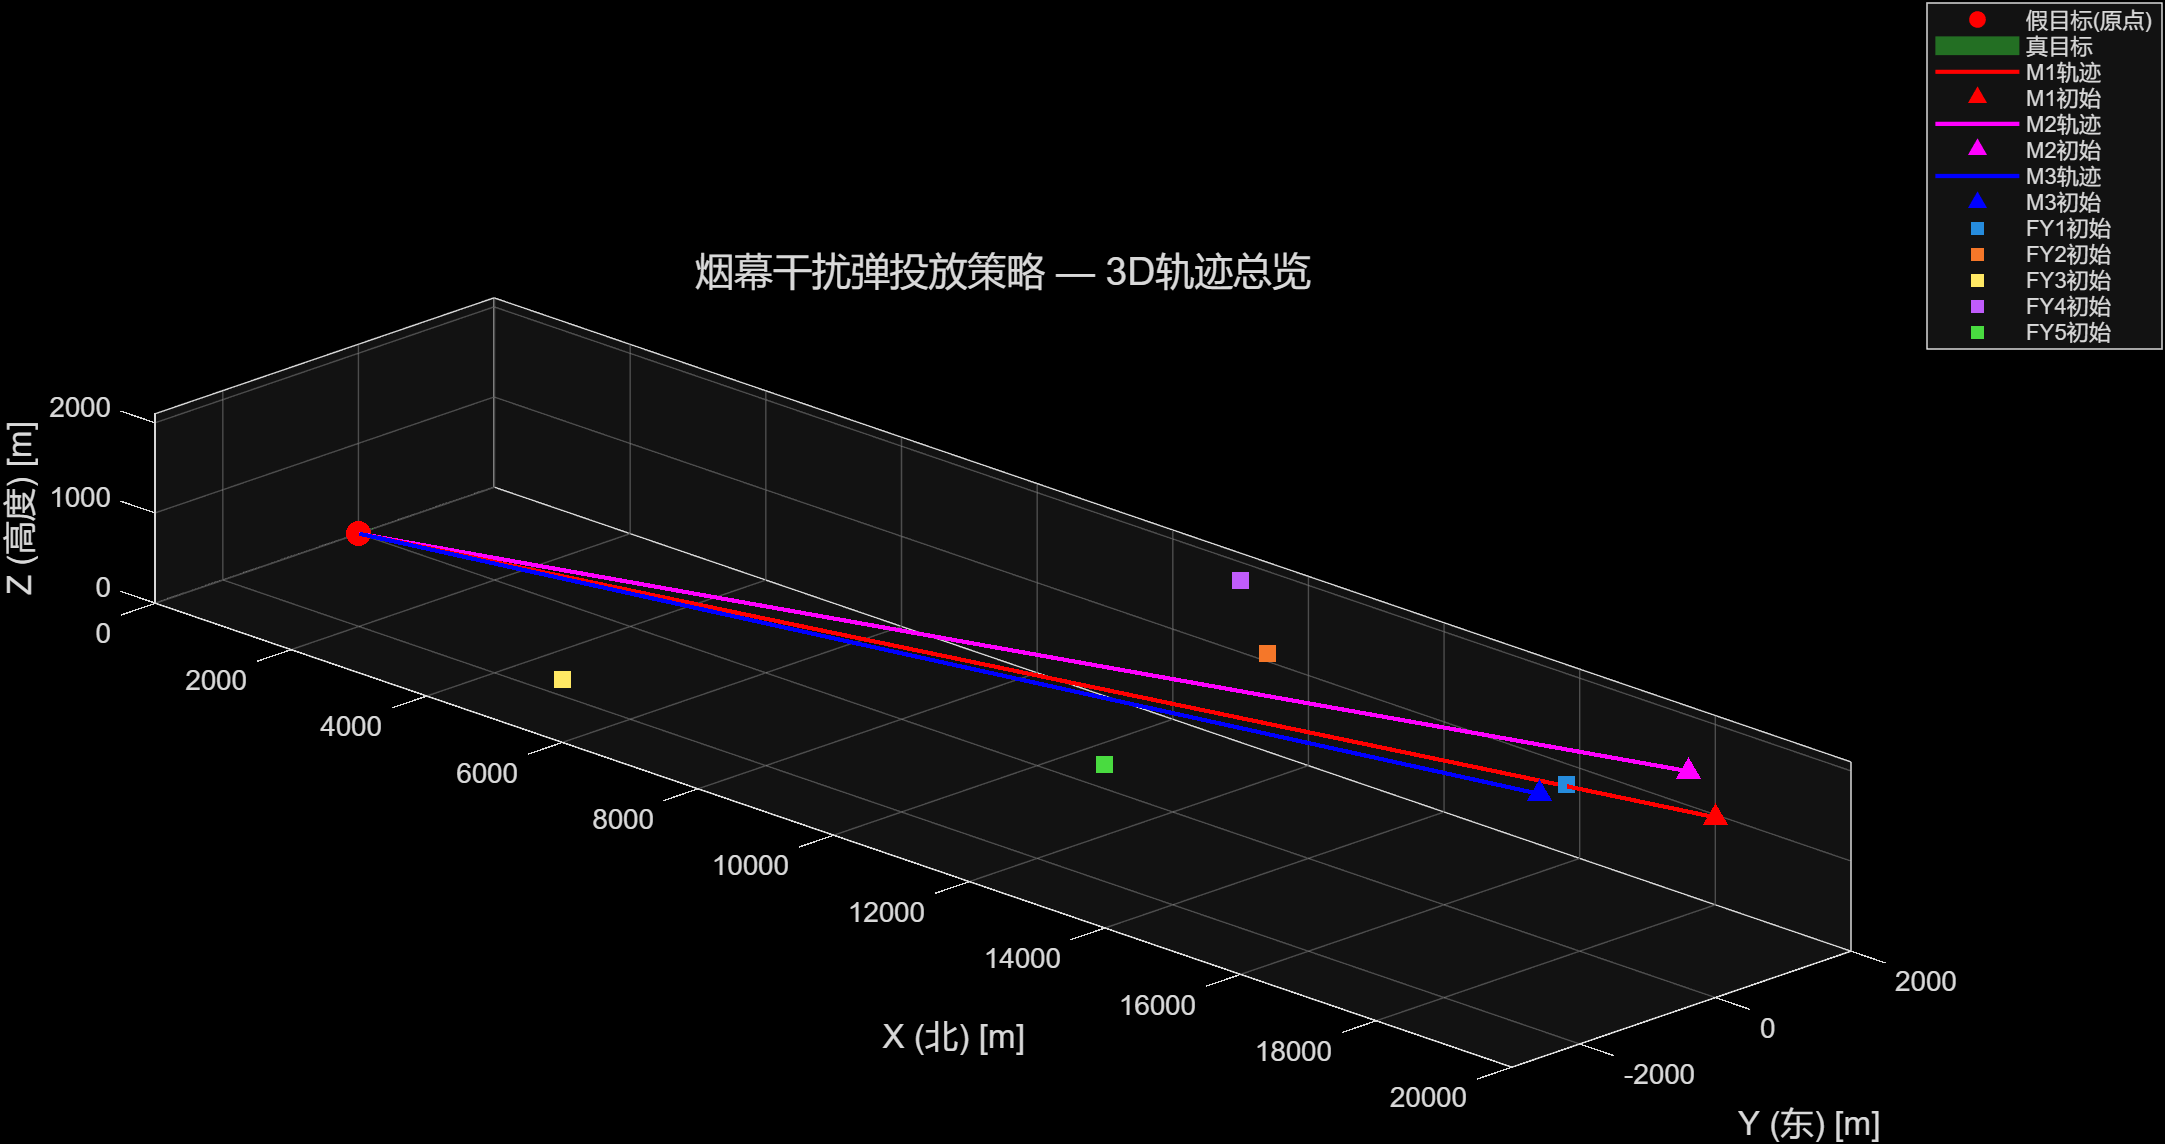
\includegraphics[width=\textwidth]{../output/figures/trajectories_overview.png}
        \caption{3D轨迹总览图}
        \label{fig:traj}
    \end{subfigure}
    \hfill
    \begin{subfigure}[b]{0.48\textwidth}
        \centering
        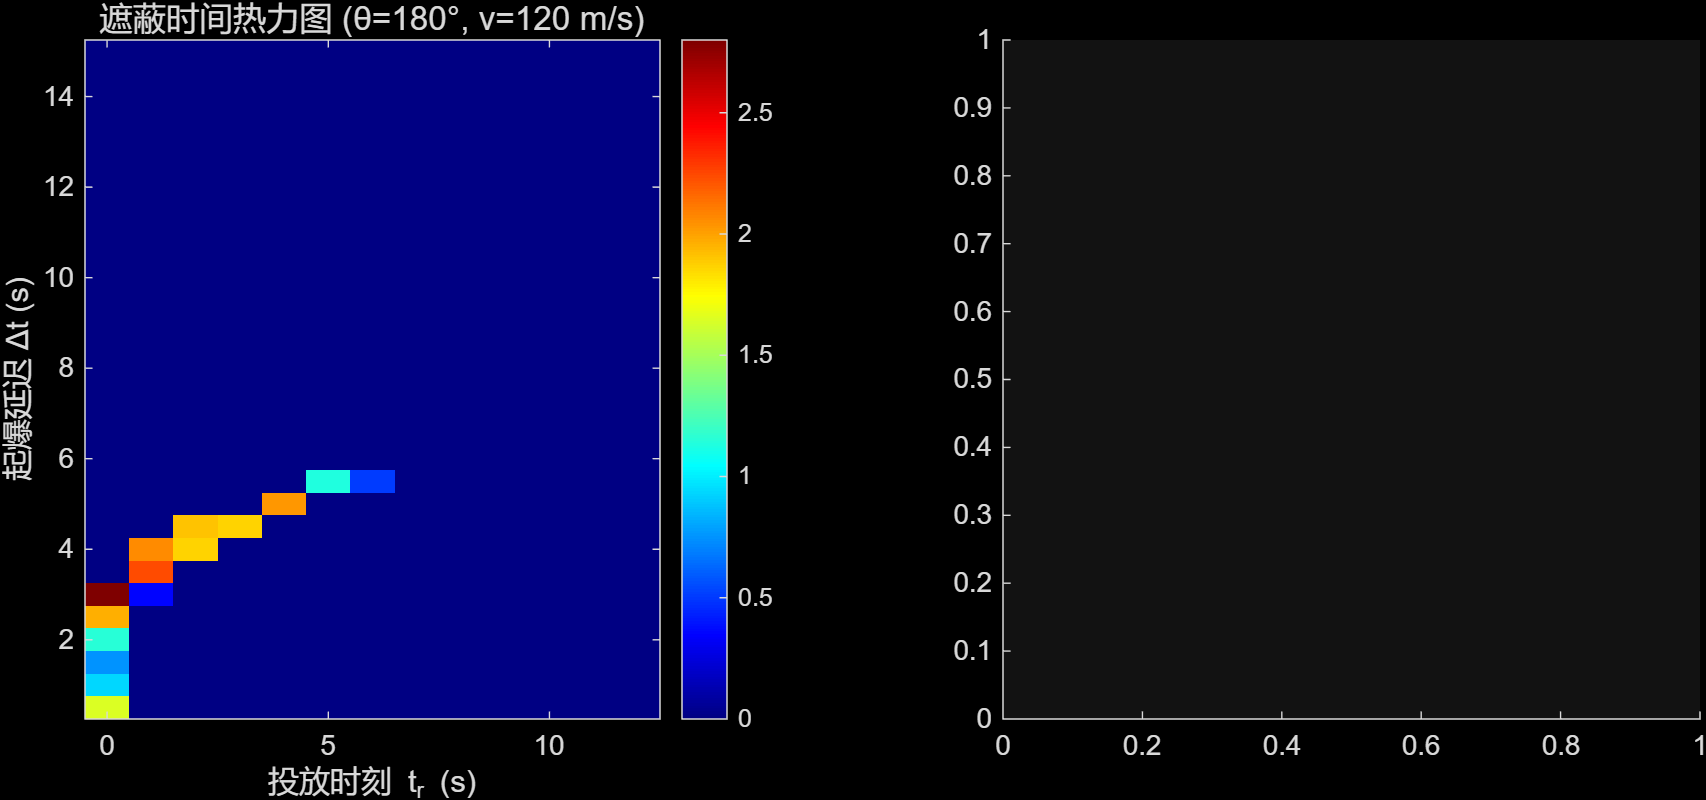
\includegraphics[width=\textwidth]{../output/figures/shielding_analysis.png}
        \caption{遮蔽效果分析图}
        \label{fig:shield}
    \end{subfigure}
    \caption{仿真结果可视化}
    \label{fig:vis}
\end{figure}

图\ref{fig:traj}展示了导弹轨迹（红色虚线）、无人机初始位置（方块标记）、真目标和假目标的空间关系。图\ref{fig:shield}以热力图形式展示了投放时刻$t_r$和起爆延迟$\Delta t$对遮蔽时间的影响，以及各问题的最优遮蔽时长对比。

图\ref{fig:conv}展示了GA优化的典型收敛过程。

\begin{figure}[H]
    \centering
    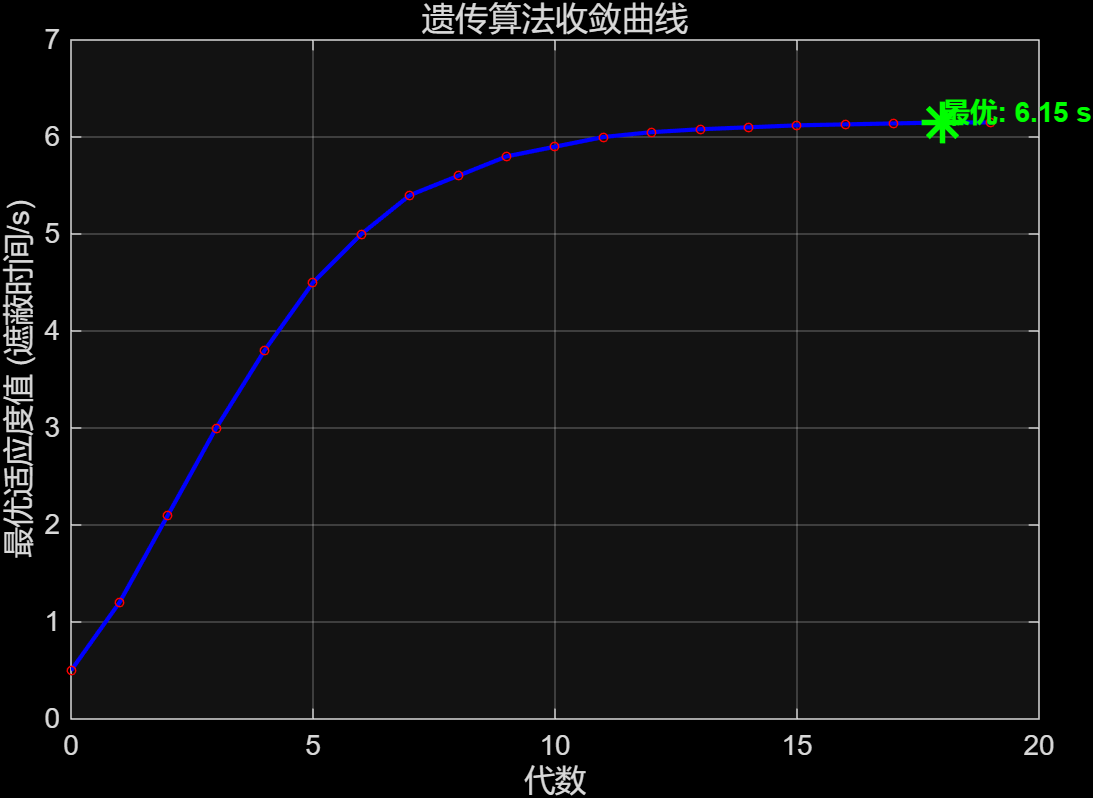
\includegraphics[width=0.6\textwidth]{../output/figures/convergence.png}
    \caption{遗传算法收敛曲线}
    \label{fig:conv}
\end{figure}
